% !TEX root = ../main.tex

%----------------------------------------
%   SECTION TITLE
%----------------------------------------
\chapter{Implementation}
\label{chap:lines_of_code}

%----------------------------------------
%   SECTION CONTENT
%----------------------------------------

In this chapter, we compare the two implementations of each app,
starting with the simplest quantitative measure:  lines of code.

\section{Lines of Code}

One criterion for comparing the DevX of two approaches is how many lines of code are required to build an application with a similar set of functionalities.
Table~\ref{tbl:lines_of_code} compares the number of lines of code for the comparison apps.

% \begin{table}
%     \centering
%     \begin{tabular}{ccc}
%         Application & TEASync & Modern Frameworks \& Libraries \\
%         Chatroom & 450 & 28\\
%         Calendar-Sync & 45 & 29\\
%     \end{tabular}
%     \caption{Caption}
%     \label{tab:my_label}
% \end{table}
\setlength{\extrarowheight}{5pt} % increase row height
\setlength{\tabcolsep}{10pt} % increase column separation

\begin{table}[]
\begin{tabular}{llrr}
% \begin{tabular}{>{\centering\arraybackslash}m{2cm}>{\centering\arraybackslash}m{2cm}>{\centering\arraybackslash}m{2cm}>{\centering\arraybackslash}m{2cm}}
\rowcolor[HTML]{C0C0C0} 
\multicolumn{2}{l|}{\cellcolor[HTML]{C0C0C0}\textbf{Applications}} & \multicolumn{1}{l|}{\cellcolor[HTML]{C0C0C0}\textbf{TEASync}} & \textbf{React \& Express} \\ \hline
\rowcolor[HTML]{EFEFEF} 
\multicolumn{4}{l}{\cellcolor[HTML]{EFEFEF}\textbf{Chatroom}} \\ \hline
          & Frontend                &     -      &    387   \\ \cline{2-4} 
          & Backend                 &     -      &    155   \\ \cline{2-4} 
          & \textbf{Total}          &      \textbf{524}     &    \textbf{542}   \\ \cline{2-4} 
\multicolumn{4}{l}{\cellcolor[HTML]{EFEFEF}\textbf{Calendar-Sync}} \\ \hline
          & Frontend                &     -      &    370   \\ \cline{2-4} 
          & Backend                 &     -      &    149   \\ \cline{2-4} 
          & \textbf{Total}          &    \textbf{269}       &    \textbf{519}   \\ \cline{2-4} 

\end{tabular}
\caption{Lines of code}\label{tbl:lines_of_code}
\end{table}


In contrast to TEASync, we divide the React application logic into two main layers, which are the backend and frontend. TEASync uses Elm to write applications, whereas modern frameworks utilize Javascript and Typescript. Additionally, modern frameworks make use of libraries, such as \lstinline{socket-io}\cite{socketio} and \lstinline{shadcn}\cite{shadcn} that reduces boilerplate code.  So differences in lines of code cannot be attributed to the frameworks alone, they depend on the different languages and library support as well.  But from the developer point of view, most of these choices are dictated by the choice of framework.  

But comparing the functionalities and features of both frameworks, they both support defining UI components as functions and having a state for components. This state can be used to persist the data between updates in the entire application state.
As shown in Table~\ref{tbl:lines_of_code},
the lines of code for the chatroom are very similar, with a slight advantage for TEASync,
whereas the distributed calendar requires half the lines of Elm code with TEASync 
compared with Javascript lines of code using React.

\section{Development Environment Setup}

The second comparison applies to developer productivity. The VSCode IDE used to develop the React applications includes extensions to enhance productivity. TEASync applications can be developed using an online IDE available at STaBL.Rock. TEASync development may require some extra efforts involving looking at language documentations and framework documentation, and lacks integration for extensions. Though there is an option to use VSCode to develop TEASync application to enhance developer experience, it still lacks extension support for the framework itself. 

Setting up the development environment for modern frameworks requires the installation of NodeJs and additional dependencies using \lstinline{npm} package manager, i.e., Express, SocketIO and React. For TEASync, developers can skip this process as the framework developer has taken care of it.

% Community and long-term support is a critical criterion while making architectural decision to choose a technology over another. Modern frameworks have a huge community support for tutorials and any issues encountered during the development phase compared to TEASync.

We further explain the architecture and implementation of the two approaches.

\section{Architecture}
\label{subsection:architecture}

\begin{figure}[ht]
    \centering
    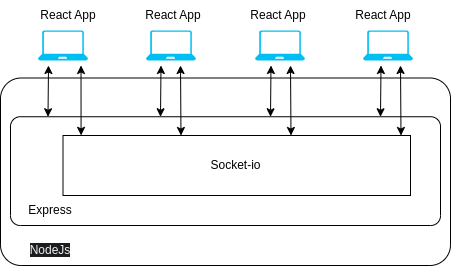
\includegraphics[width=0.8\textwidth]{diagrams/App Architecture.png}
    \caption{High-Level Application Architecture}
    \label{fig:ReactFlow}
\end{figure}

As shown in Figure~\ref{fig:ReactFlow}, clients use the React application to communicate with the Express and SocketIO server on the back end to sync the data among them. Clients join a ``room'' to participate in a session, which is managed at the server level. 
This two-way dataflow contrasts with the one-way flow flow in Figure~\ref{fig:teasync-architecture}, 
which follows from the purity of Elm versus the mutability of Javascript data.

Local updates propagate update requests to the server and the server verifies the requests and finds the room associated with the request.
After validation, the server emits new state for the application to all clients in the room.
This flow of information achieves the synchronization of the state to multiple clients.

% Few code snippets and patterns from both applications will be discussed further.
We will compare the experience of implementing state management, session management, data synchronization and communication flow using TEASync and Express and React.

\subsection{State Management}

Both applications rely on local and global states to store the data, which will be subsequently used in different parts of the application. The states data can be modified with the actions from user and server responses. 

% \textbf{Ease of defining and updating states} 

Defining and managing the application state is a trivial operation for any modern complex web applications. Various techniques and best practices are available to tame the complexity of state management. We used the Redux\cite{redux} library for the state management in our application to maintain the application’s global state and React’s built-in state hook for local state management. 

\begin{lstlisting}[language=Java, caption=Calendar State in React Application, label=lst:java, mathescape=true]
export interface CustomizedAppConfig {
    isLoggedIn: boolean,
    username: string,
    userType: "admin" | "user" | "unknown"
    sessionId: string
}
\end{lstlisting}

TEASync simplifies application state management by eliminating the need for additional libraries or setup. With TEASync, you can define your state of application as local and global models and pass them directly to the application configuration. This approach avoids common pitfalls and eliminates the steep learning curve associated with state-management libraries. Moreover, TEASync streamlines state management by removing the need for separate components to fetch and update values, making rapid prototyping a breeze.

\begin{lstlisting}[language=Java, caption=TEASync Calendar State, label=lst:java, mathescape=true]
//Local State
initLocal : LocalModel
initLocal = { time = 0, dragState = Waiting }

//Global State
initGlobal : GlobalModel
initGlobal = { calendar = Dict.empty }

//Application Configuration
appConfig =
    simpleAppConfig
    { 
        initLocal = initLocal
        , initGlobal = initGlobal
        , localUpdate = localUpdate
        , globalUpdate = globalUpdate
        , view = view
        , codecGlobalModel = JSON Codec.Encoders.encodeGlobalModel Codec.Decoders.decodeGlobalModel
        , codecGlobalMsg = JSON Codec.Encoders.encodeGlobalMsg Codec.Decoders.decodeGlobalMsg
    }

\end{lstlisting}

% \subsection{UI Request for Authentication and Session Creation}
\subsection{Session Management}
Session Management is a method used to temporarily save user information on the server. It starts when a user logs into the application and remains until the user logs out of the application or shuts down the machine. It is a sequence of network HTTP request and response transactions associated with the same user.

% =======================================================
TEASync implements a WebSocket server using the IHP (Integrated Haskell Platform) framework. The session management is handled through the \lstinline{TSWSServerController} and \lstinline{TSWSServerState} data types.
Here is a breakdown of the session management:

\textbf{\lstinline{TSWSServerController}}: This data type represents the state of a single WebSocket connection. It can be in one of two states:

\begin{itemize}
    \item \lstinline{WaitingToConnect}: The initial state before a client connects.
    \item \lstinline{ClientConnected}: The state after a client connects, containing the server ID, client ID, and a boolean indicating whether the client is headless (i.e., a server-side client).
\end{itemize}

\textbf{\lstinline{TSWSServerState}}: This data type represents the state of the entire WebSocket server. It contains the following fields:

\begin{itemize}
    \item \lstinline{nextId}: The next available client ID.
    \item \lstinline{clientMap}: A map of server IDs to a set of connected client IDs.
    \item \lstinline{clientChannels}: A map of client IDs to their corresponding WebSocket queues (of type \lstinline{WSClientQueue}).
    \item \lstinline{headlessClientIDs}: A map of server IDs to their corresponding headless client IDs.
    \item \lstinline{serverModels}: A map of server IDs to their corresponding models (stored as JSON values).
    \item \lstinline{unstoredModels}: A set of server IDs with unstored models.
    \item \lstinline{unstoredModelThreadStarted}: A boolean indicating whether the thread for storing unstored models has been started.

\end{itemize}

% =======================================================

The second approach creates a server using the Express library and CORS. It implements session management using a simple in-memory store. Here is a breakdown of the session management aspects:

\begin{itemize}
    \item User Sessions: The \lstinline{userSessions} Map stores the session ID for each user. When a user logs in, a new session ID is generated and stored in this map.
    \item Session Participants: The \lstinline{sessionParticipants} array stores the session details, including the participants (users) in each session.
    \item Session Messages: The \lstinline{sessionMessages} Map stores the messages for each session.
    \item Login: When a user logs in, the server checks the credentials and generates a new session ID if the user is valid. The session ID is then stored in the \lstinline{userSessions} map.
    \item Session Creation: When a new session is created, the server generates a new session ID and stores the participants in the \lstinline{sessionParticipants} array.
    \item Session Management: When a user connects or disconnects, the server updates the session information accordingly.
    \item Chatroom: The server creates a new namespace for each chatroom (session) and handles socket events specific to that chatroom.
\end{itemize}

For chatroom application, the authorized users can create a chatroom for a defined set of users. 

\textbf{Authentication}


% \textbf{To be filled for chatroom TEASync Application}
TEASync Chatroom application requires you to create an Admin user to start a session. This includes entering admin credentials, adding credentials for users to login. Credentials are stored in a local model of the application and we need to provide the validation logic for users and admin.

The following is a breakdown of the authentication in the chatroom application.
\begin{itemize}
    \item \lstinline{LoginUserInput}: When a user inputs their username, the \lstinline{LoginUserInput} message is triggered. The code updates the local model's state by storing the username
    \item \lstinline{LoginPassInput}: When a user inputs their password, the \lstinline{LoginPassInput} message is triggered. The code updates the local model's state by storing the password
    \item \lstinline{SubmitAdmin}: When the admin submits their credentials, the code checks if the input fields are empty. If they are, it displays an error message. If not, it performs a task to register the admin and updates the local model's state to enter new logins
    \item \lstinline{AdminSet}: When the admin is set, the code checks if the returned admin credentials match the expected credentials. If they do, it updates the local model's state to enter new logins. If not, it displays an error message
    \item \lstinline{TryLogin}: When the user attempts to log in, the code trims the input username and password, updates the local model's state to waiting for login, and performs a task to send the login credentials
\end{itemize}
\vspace{1.5em}

\begin{lstlisting}[language=Java, caption= TEASync Admin User Setup, label=lst:java, mathescape=true]
localUpdate msg localModel globalModel = 
  case msg of
    ...
    LoginUserInput user   -> ({ localModel | state = case localModel.state of
                                                      Login _ pass txt -> Login user pass txt
                                                      _ -> localModel.state 
                              }, Cmd.none, Cmd.none)
                              
    LoginPassInput pass   -> ({ localModel | state = case localModel.state of
                                                      Login user _ txt -> Login user pass txt
                                                      _ -> localModel.state 
                              }, Cmd.none, Cmd.none)

    SubmitAdmin ->
        case localModel.state of
            SettingAdmin admin adminPass _ -> 
              if (String.isEmpty admin || String.isEmpty adminPass) then
                ( { localModel | state = SettingAdmin "" "" "Please fill out the required fields!" }
                  , Cmd.none, Cmd.none )
              else
                ( { localModel | state = EnterNewLogins admin "Enter initial logins." "" }
                , Cmd.none, Task.perform (RegisterAdmin admin) (Task.succeed adminPass) )
            _ ->
              ( localModel, Cmd.none, Cmd.none )
    
    AdminSet adminReturned ->
        case localModel.state of
            WaitingForAuth admin adminPass _ ->
              if adminReturned == admin++adminPass then
                ( { localModel | state = EnterNewLogins admin "Enter initial logins." "" }
                , Cmd.none, Cmd.none )
              else
                ( { localModel | state = SplashScreen "Admin already set!" }
                , Cmd.none, Cmd.none )
            _ ->
              ( localModel, Cmd.none, Cmd.none )
    TryLogin ->
        case localModel.state of
            Login user pass _ ->
              let
                loginUsername = user
                          |> String.trim
            
                loginPass = pass
                          |> String.trim
                          
              in
                ( { localModel | state = WaitingForLogin user }
                , Cmd.none, Task.perform (SendLogin loginUsername) (Task.succeed loginPass) )
            _ ->
              ( localModel, Cmd.none, Cmd.none )
\end{lstlisting}

For the second approach, Authentication calls are made from the React application to the backend Express server to authenticate a user. This logic can be implemented on the React application, however this is not recommended.

Following the initialization, we defined our business logic for authentication and session management for the Express server. 

\begin{lstlisting}[language=Java, caption=Authentication API Endpoints, label=lst:java, mathescape=true]
app.post("/login/admin", (request, response) => {
    const { username, password } = request.body;
    const user = users.find(user => user.username === username && user.password === password);
    if (user) {
        response.json({ message: 'Login successful' });
    } else {
        response.status(401).json({ error: 'Invalid username or password' });
    }
})

app.post("/login/participant", (request, response) => {
    const { username, password, sessionId } = request.body;
    const r_session = sessionParticipants.find((session) => session.id == sessionId)

    if(!r_session){
        response.status(401).json({ error: 'Invalid session' });
    }

    const user = r_session?.participants.find(user => user.username === username && user.password === password);
    if (user) {
        response.json({ message: 'Login successful' });
    } else {
        response.status(401).json({ error: 'Invalid username or password' });
    }
})
\end{lstlisting}

The above code snippet shows two API endpoints to handle authentication. First API endpoint is to authenticate the user with admin access, whereas second API endpoint is used by other participants with no special roles. 

\begin{lstlisting}[language=Java, caption=Authentication Request, label=lst:java, mathescape=true]
try {
    const response = await fetch('http://localhost:3002/login/admin', {
        method: 'POST',
        headers: {
            'Content-Type': 'application/json'
        },
        body: JSON.stringify(ob_json)
    });

    if (!response.ok) {
        throw new Error('Network response was not ok');
    }

    dispatch(setUserInfo({username:  username, userType: "admin", isLoggedIn: true}));    
    router.push('/session/new');
\end{lstlisting}

For the Chatroom application, if an user is successfully authenticated, the user is then redirected to a new session page to enter the details of the other users to join the chatroom.

Similarly, for Calendar-sync app the user is redirected to the main calendar app and this session can be shared among different users to view and update the calendar.

\subsection{Data Synchronization}

For TEASync, application-specific types such as local and global messages can be defined in a single file Types.elm. 

\begin{lstlisting}[language=Haskell, caption=Local and Global messages in Types.elm, label=lst:haskell, mathescape=true]
type LocalMsg 
    = Tick Float GetKeyState
    | MouseDownToAddMeetingAt (Float,Float)
    | MouseDownToAdjustStartAt (Day,Start) (Float,Float)
    | MouseDownToAdjustStopAt (Day,Start) (Float,Float)
    | MouseMoveAt (Float,Float)
    | MouseUp
    | MouseLeave

type GlobalMsg
  = AddMeetingAt Meeting (Float,Float)
  | ChangeMeetingStart (Day,Start) Meeting (Float,Float) 
  | ChangeMeetingEnd (Day,Start) Meeting (Float,Float)
  | DeleteMeeting (Day,Start)
  | TapToToggleAttendance (Day,Start) Person
  | TapToToggleLocation (Day,Start)

\end{lstlisting}


For synchronization of messages across the clients, the server handles the message synchronization and no custom implementation is required. This reduces the complexity of understanding a particular technology and helps developers focus on application logic rather than worrying about the application infrastructure.

The data synchronization for TEASync backend server works as follows:
\begin{itemize}
    \item When a new client connects, a new \lstinline{TSWSServerController} is created in the \lstinline{WaitingToConnect} state.
    \item Once the client is authenticated and connected, the controller transitions to the \lstinline{ClientConnected} state, storing the server ID, client ID, and headless status.
    \item The \lstinline{TSWSServerState} is updated to reflect the new connection, adding the client ID to the \lstinline{clientMap} and creating a new \lstinline{WSClientQueue} for the client.
    \item When a client sends a message, it is received by the server and processed according to the \lstinline{WSClientCmd} data type.
    \item The server can send messages to clients using the \lstinline{WSClientCmd} data type, which is serialized to JSON and sent over the WebSocket connection.
\end{itemize}

Note that this implementation uses STM (Software Transactional Memory) for concurrent access to the \lstinline{TSWSServerState} and \lstinline{WSClientQueue} data structures, ensuring thread safety and atomicity by default.

On the application side, the developer only needs to implement the logic to react to events as described without worrying about serialization and de-serialization of data and type inference.

\begin{lstlisting}[language=Java, caption=Global State Update, label=lst:java, mathescape=true]
globalUpdate : GlobalMsg -> GlobalModel -> GlobalModel
globalUpdate msg globalModel =
  case msg of
    AddMeetingAt meeting xy -> 
      { globalModel | calendar = Dict.insert (pos2time xy) meeting globalModel.calendar}
    ChangeMeetingStart oldDayStart newMeeting xy ->
      { globalModel | calendar = globalModel.calendar
                                   |> Dict.remove oldDayStart
                                   |> Dict.insert (pos2time xy) newMeeting
...
\end{lstlisting}

The second approach also relies WebSockets using the \lstinline{socket-io} library to communicate with the backend systems. The apps, when loaded, try to establish the connection with backend socket server using the following code.

\begin{lstlisting}[language=Java, caption=New Connection Initialization, label=lst:java, mathescape=true]
if (socket) {
    socket.emit('joinRoom', params.id);
    socket.on('updateEvents', (newEvents) => {
        setEvents(newEvents.map((event) => ({
            ...event,
            start: new Date(event.start),
            end: new Date(event.end)
        })));
    });
    socket.on('allEvents', (allEvents: MyEvent[]) => {
        setEvents(allEvents.map((event) => ({
            ...event,
            start: new Date(event.start),
            end: new Date(event.end)
        })));
    })
}
\end{lstlisting}

The code snippet above is from the Calendar-sync application, which demonstrates the handling of socket connections and event reactions. Upon successful connection, the application reacts to specific events, processing data accordingly. When the \lstinline{updateEvents} event is received, a new set of calendar events is updated, modifying the local state containing the event list. Additionally, the \lstinline{allEvents} event is triggered when a new user joins the session, updating local events with existing session events.

\begin{lstlisting}[language=Java, caption=WebSocket Events, label=lst:java, mathescape=true]
io.on('connection', (socket) => {
    let roomId;
     socket.on('createRoom', (payload) => {
        activeRooms[payload.sessionId] = { users: [payload.username], messages: [] };
        socket.join(payload.sessionId);
        socket.emit('roomCreated', payload);
    });

    socket.on('joinRoom', (payload) => {
        const room = activeRooms[payload];
        if(!room){
            activeRooms[payload] = {events:[]};
            console.log(`New room created: ${payload}`);
            activeRooms[payload].userCount = 1;
        }
        if (room) {
            socket.join(payload);
            const events = activeRooms[payload].events;
            socket.emit('allEvents', events);
            activeRooms[payload].userCount++;
        }
    });

    socket.on('updateEvents', (payload) => {
        const { sessionId, newEvents} = payload;
        const room = activeRooms[sessionId];
        if (room) {
            room.events= newEvents;
            io.to(sessionId).emit('updateEvents', newEvents);
        }
    });

    socket.on('disconnect', () => {
        console.log(`Disconnecting...`);
    });
});
\end{lstlisting}

The code snippet above illustrates the synchronization logic for socket connections. When an authenticated user initiates a session, the server receives a \lstinline{createRoom} event. Each session is assigned a unique room ID that serves as an identifier for subsequent requests related to that session. Notably, this room ID also enables the creation of 'rooms' in \lstinline{socket-io}, allowing for targeted communication with specific clients. In \lstinline{socket-io}, rooms act as arbitrary channels that sockets can join or leave, facilitating the broadcast of events to select clients\cite{socketio}.

\begin{figure}[ht]
    \centering
    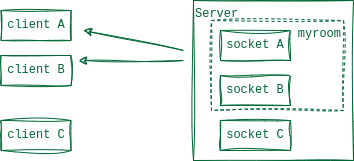
\includegraphics[width=0.8\textwidth]{diagrams/SocketIORooms.png}
    \caption{SocketIO Rooms}
    \label{fig:enter-label}
\end{figure}

This mechanism enables us to group clients together and publish events, simplifying our implementation and avoiding the complexity of developing our own solution.

\begin{lstlisting}[language=Java, caption=Data Synchronization in React Component, label=lst:java, mathescape=true]
function sendMessage(formData) {
        const json_ob = {
            sender: username,
            roomId: sessionId,
            message: formData.get("message")
        }
        if(socket)
            socket.emit('sendMessage', json_ob);
    }

useEffect(() => {
    if (socket) {
        if (userType == 'user') {
            socket.emit('joinRoom', { sessionId, username });
        }
        else if (userType == 'admin') {
            socket.emit('createRoom', { sessionId, username })
        }
        socket.on('joinedRoom', (data) => {
            setChatHistory((previousState) => {
                return data.chatHistory
            });
        });
        socket.on('newMessage', (data) => {
            setChatHistory((previousChatHistory) => {
                return [...previousChatHistory, data];
            })
        });
        socket.on('userJoined', (data) => {
            ...
        });
        socket.on('userLeft', (data) => {
            ...
        });
    }
\end{lstlisting}

The code snippet above illustrates various events emitted by the frontend for the Chatroom application. If the current user is an admin, the frontend sends a request to the backend server to initiate a new session. If the current user is a normal participant, the socket request connects to the created room.

The \lstinline{sendMessage} method handles the click event on the 'send' button, sending user-entered messages in the chat box to the server. This process updates the local message history and sends the updated list to the server. When the \lstinline{newMessage} event occurs, other connected clients receive these updates from the server and their local state is updated. Additionally, the frontend application receives notifications for events such as user join/leave via the \lstinline{userJoined} and \lstinline{userLeft} events, respectively.

This approach requires familiarity and expertise with the library, which comes with a moderately steep learning curve. However, TEASync excels over modern approaches as it allows programmers to prototype without committing to a specific technology beforehand.


% \subsection{Backend: Express and Socket Server}
% \subsection{Communication Flow}
% Backend of both applications built using Express and Socket-io running in a NodeJs environment. It consist of endpoints to handle the authentication, new session request and socket server to sync data across the connected clients.

% Web socket, a communication protocol that supports full-duplex communication channels over a single, long-lived connection between the client and the server, is used to emit events whenever a local state is updated at the client end. These changes are propagated to the clients as programmed.

% \begin{lstlisting}
% const express = require('express');
% const http = require('http');
% const socketIo = require('socket.io');
% const cors = require('cors');
% const bodyParser = require('body-parser');


% const app = express();
% app.use(cors());
% const server = http.createServer(app);
% const port = 5050
% const io = socketIo(server, {
%     cors: {
%         origin: "*", 
%         methods: ["GET", "POST"]
%     }
% });
% ...
% server.listen(port, () => {
%     console.log(`Server is running on port ${port}`);
% });
% \end{lstlisting}

% Above code snippet show how the backend server is initialized. An Express application acts as http web server with a socket server attached. The ports and other configuration such as accepted HTTP methods and CORS, port can be configured as per the requirements.


% \blindtext[2]

% \begin{figure}[ht]
%     \centering
%     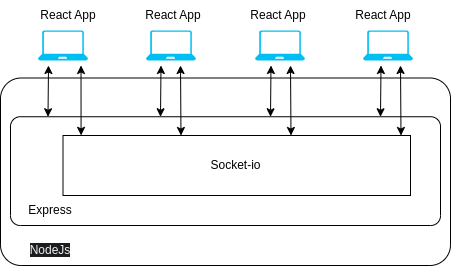
\includegraphics[width=0.8\textwidth]{diagrams/App Architecture.png}
%     \caption{Caption}
%     \label{fig:enter-label}
% \end{figure}